\subsection{Surrogate Gradients During Training}
We now analyze the effect of surrogate gradient slope choices on both fully supervised, Behavioral Cloning (BC), and fully online training algorithms, TD3 \cite{fujimoto2018addressing}. To eliminate the effect of the warm-up during training for this analysis, we do the following. We stack a history of observations, process multiple forward passes per observation and reset the SNN in between subsequent actions, similar to previous RL implementations for SNNs. The dataset used for BC has been gathered with the privileged actor introduced in \autoref{sub:seq_snn}. The following experiments do not use a reward curriculum, nor learn from the temporal dimension.

While slope choice barely affects supervised learning, online RL strongly prefers shallower slopes whose induced gradient noise enhances exploration, similar to parameter noise \cite{plappert2017parameter}, albeit with higher variability across runs. Poor intermediate updates can corrupt the replay buffer with low-quality experiences, hindering convergence. Shallower slopes introduce noise in the policy update, and therefore heighten this risk, making training less stable. 

We observe that scheduled slope settings firstly reduces the number of epochs to reach a reward of $100$ by a factor $\times 4.5$ compared to steeper slopes. Secondly, final performance of the trained agents lie in the same regime as fixed slope experiments.
\begin{figure*}[h!]
    \centering
    \begin{subfigure}[b]{0.49\textwidth}
        \centering
        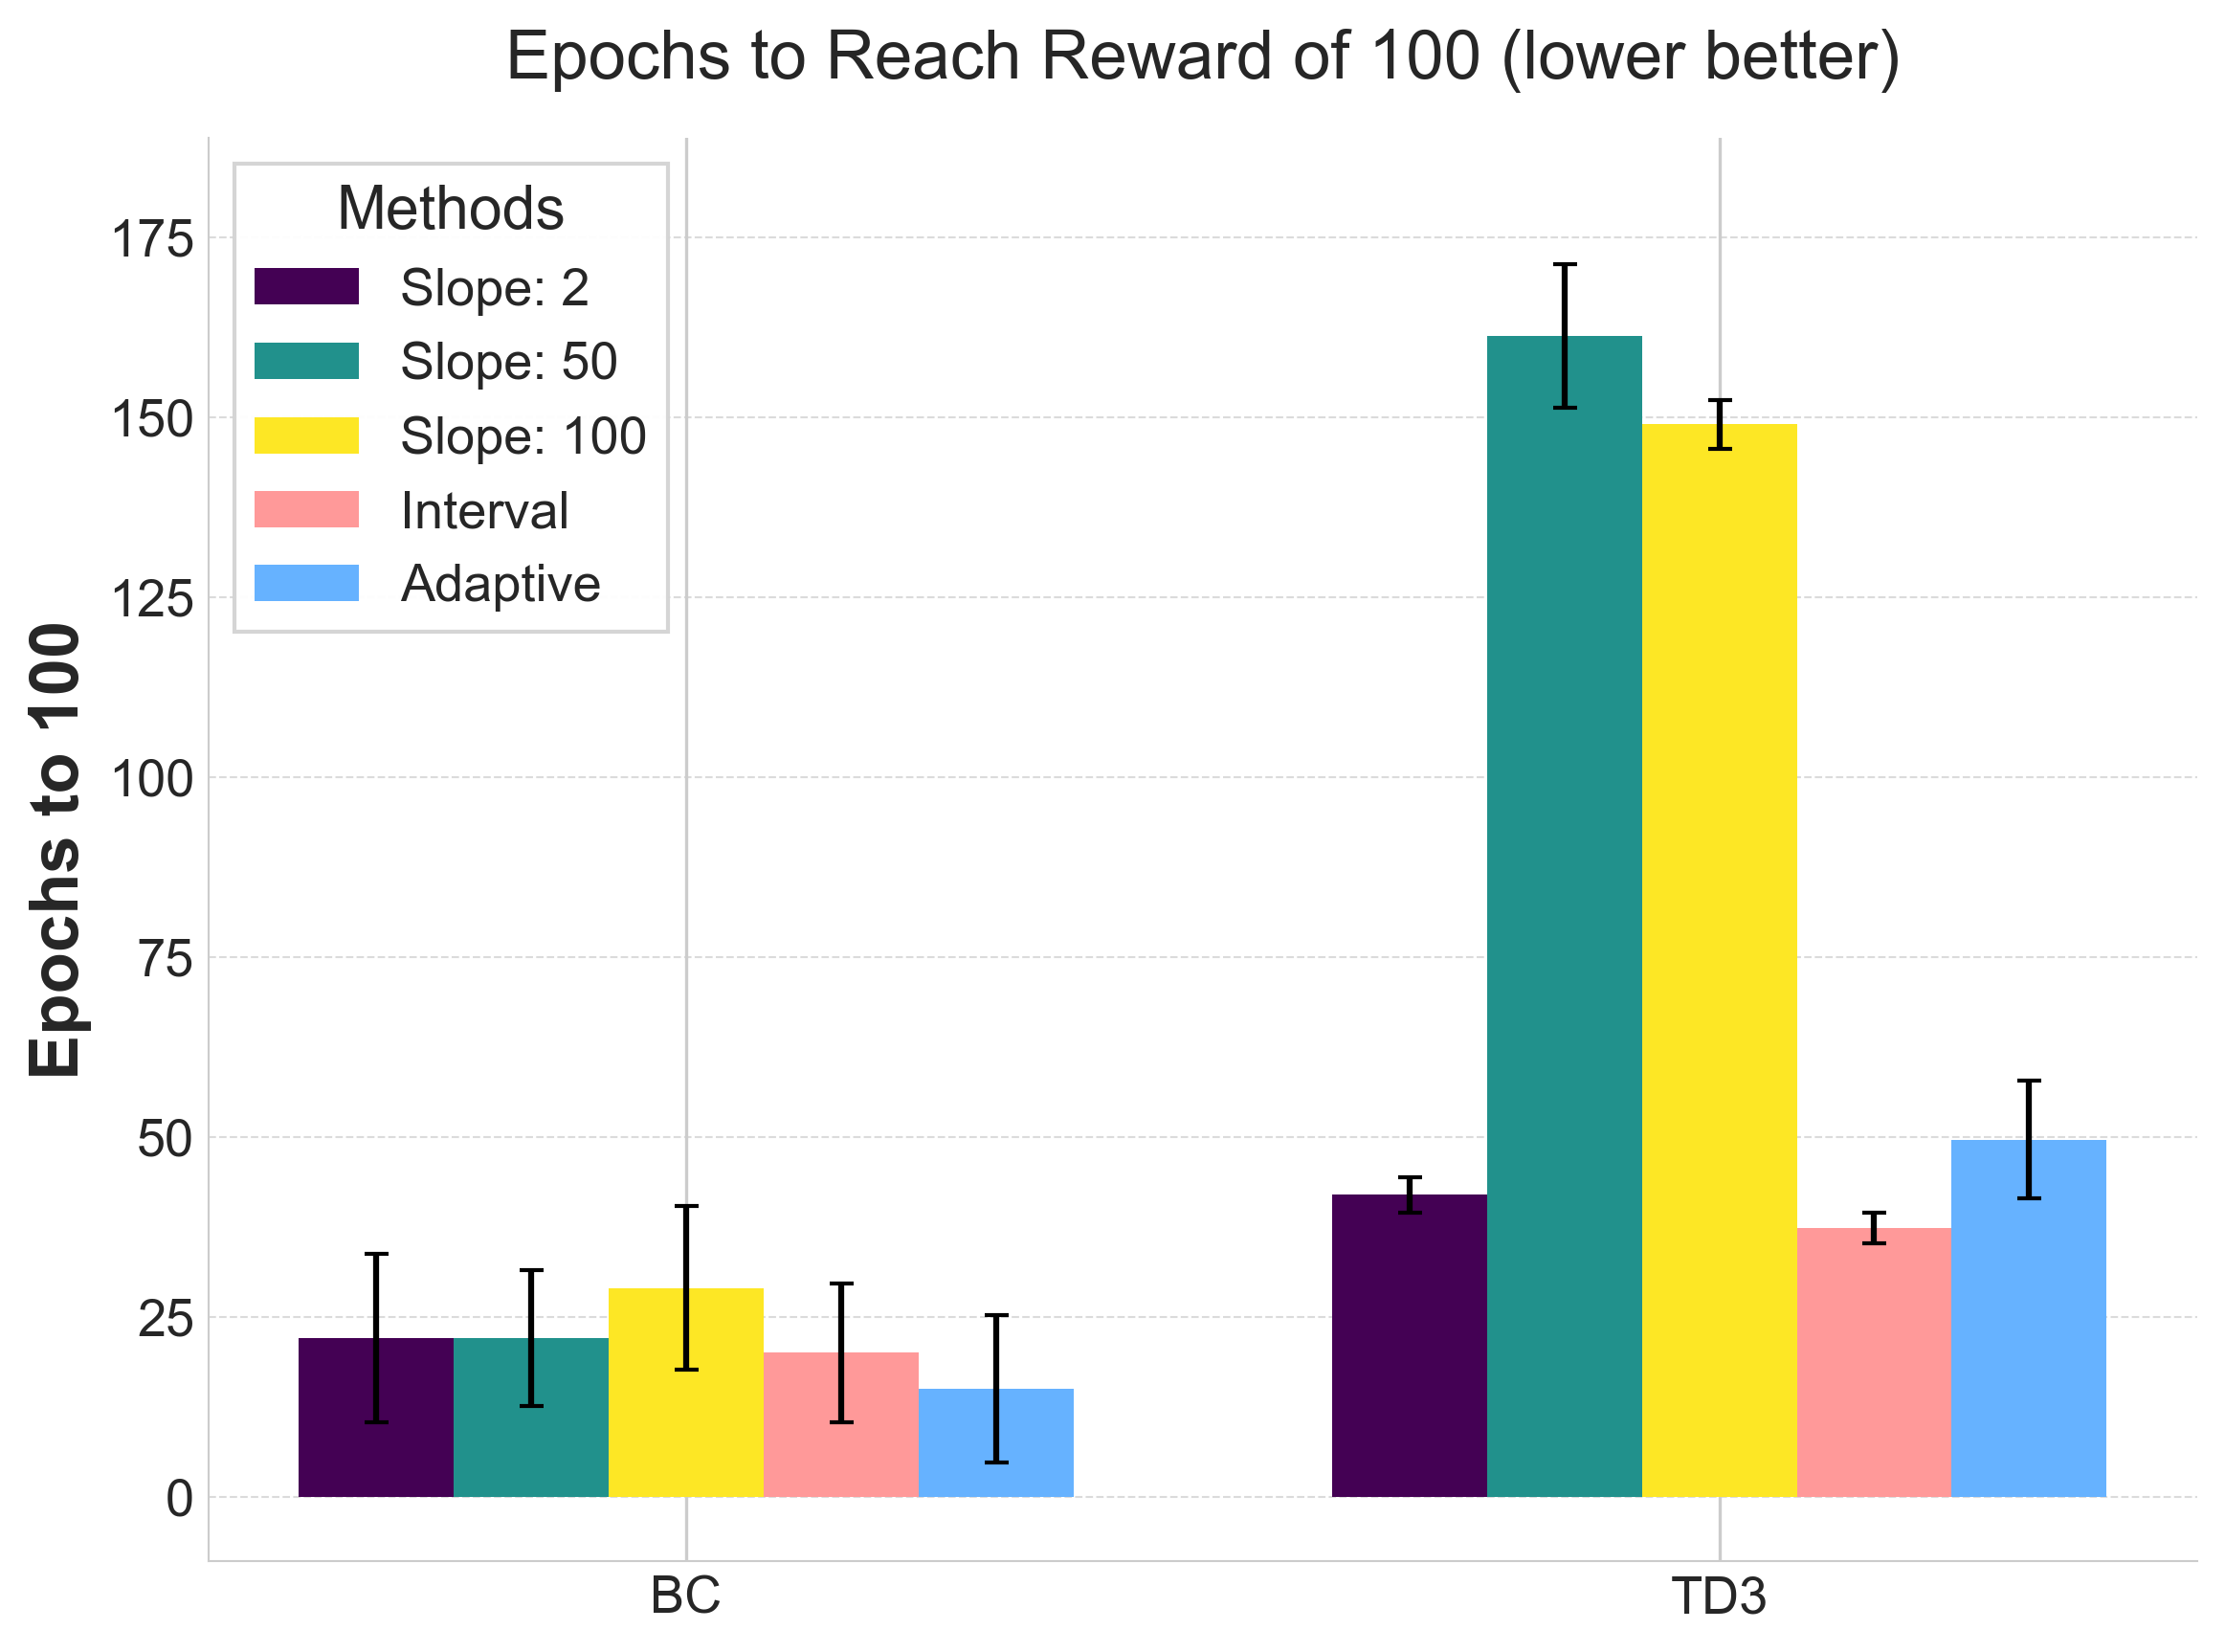
\includegraphics[width=\textwidth]{figures/neurips_time_to_100_plot.png}
        \caption{In BC, convergence speed is largely unaffected by the surrogate slope, as the noisier updates from shallow slopes are compensated by broader gradient propagation. In contrast, RL benefits significantly from shallower slopes, which enhance exploration through gradient noise. Scheduled slopes achieve competitive convergence speeds without manual tuning.}
        \label{fig:time_to_100_plot}
    \end{subfigure}
    \hfill
    \begin{subfigure}[b]{0.49\textwidth}
        \centering
        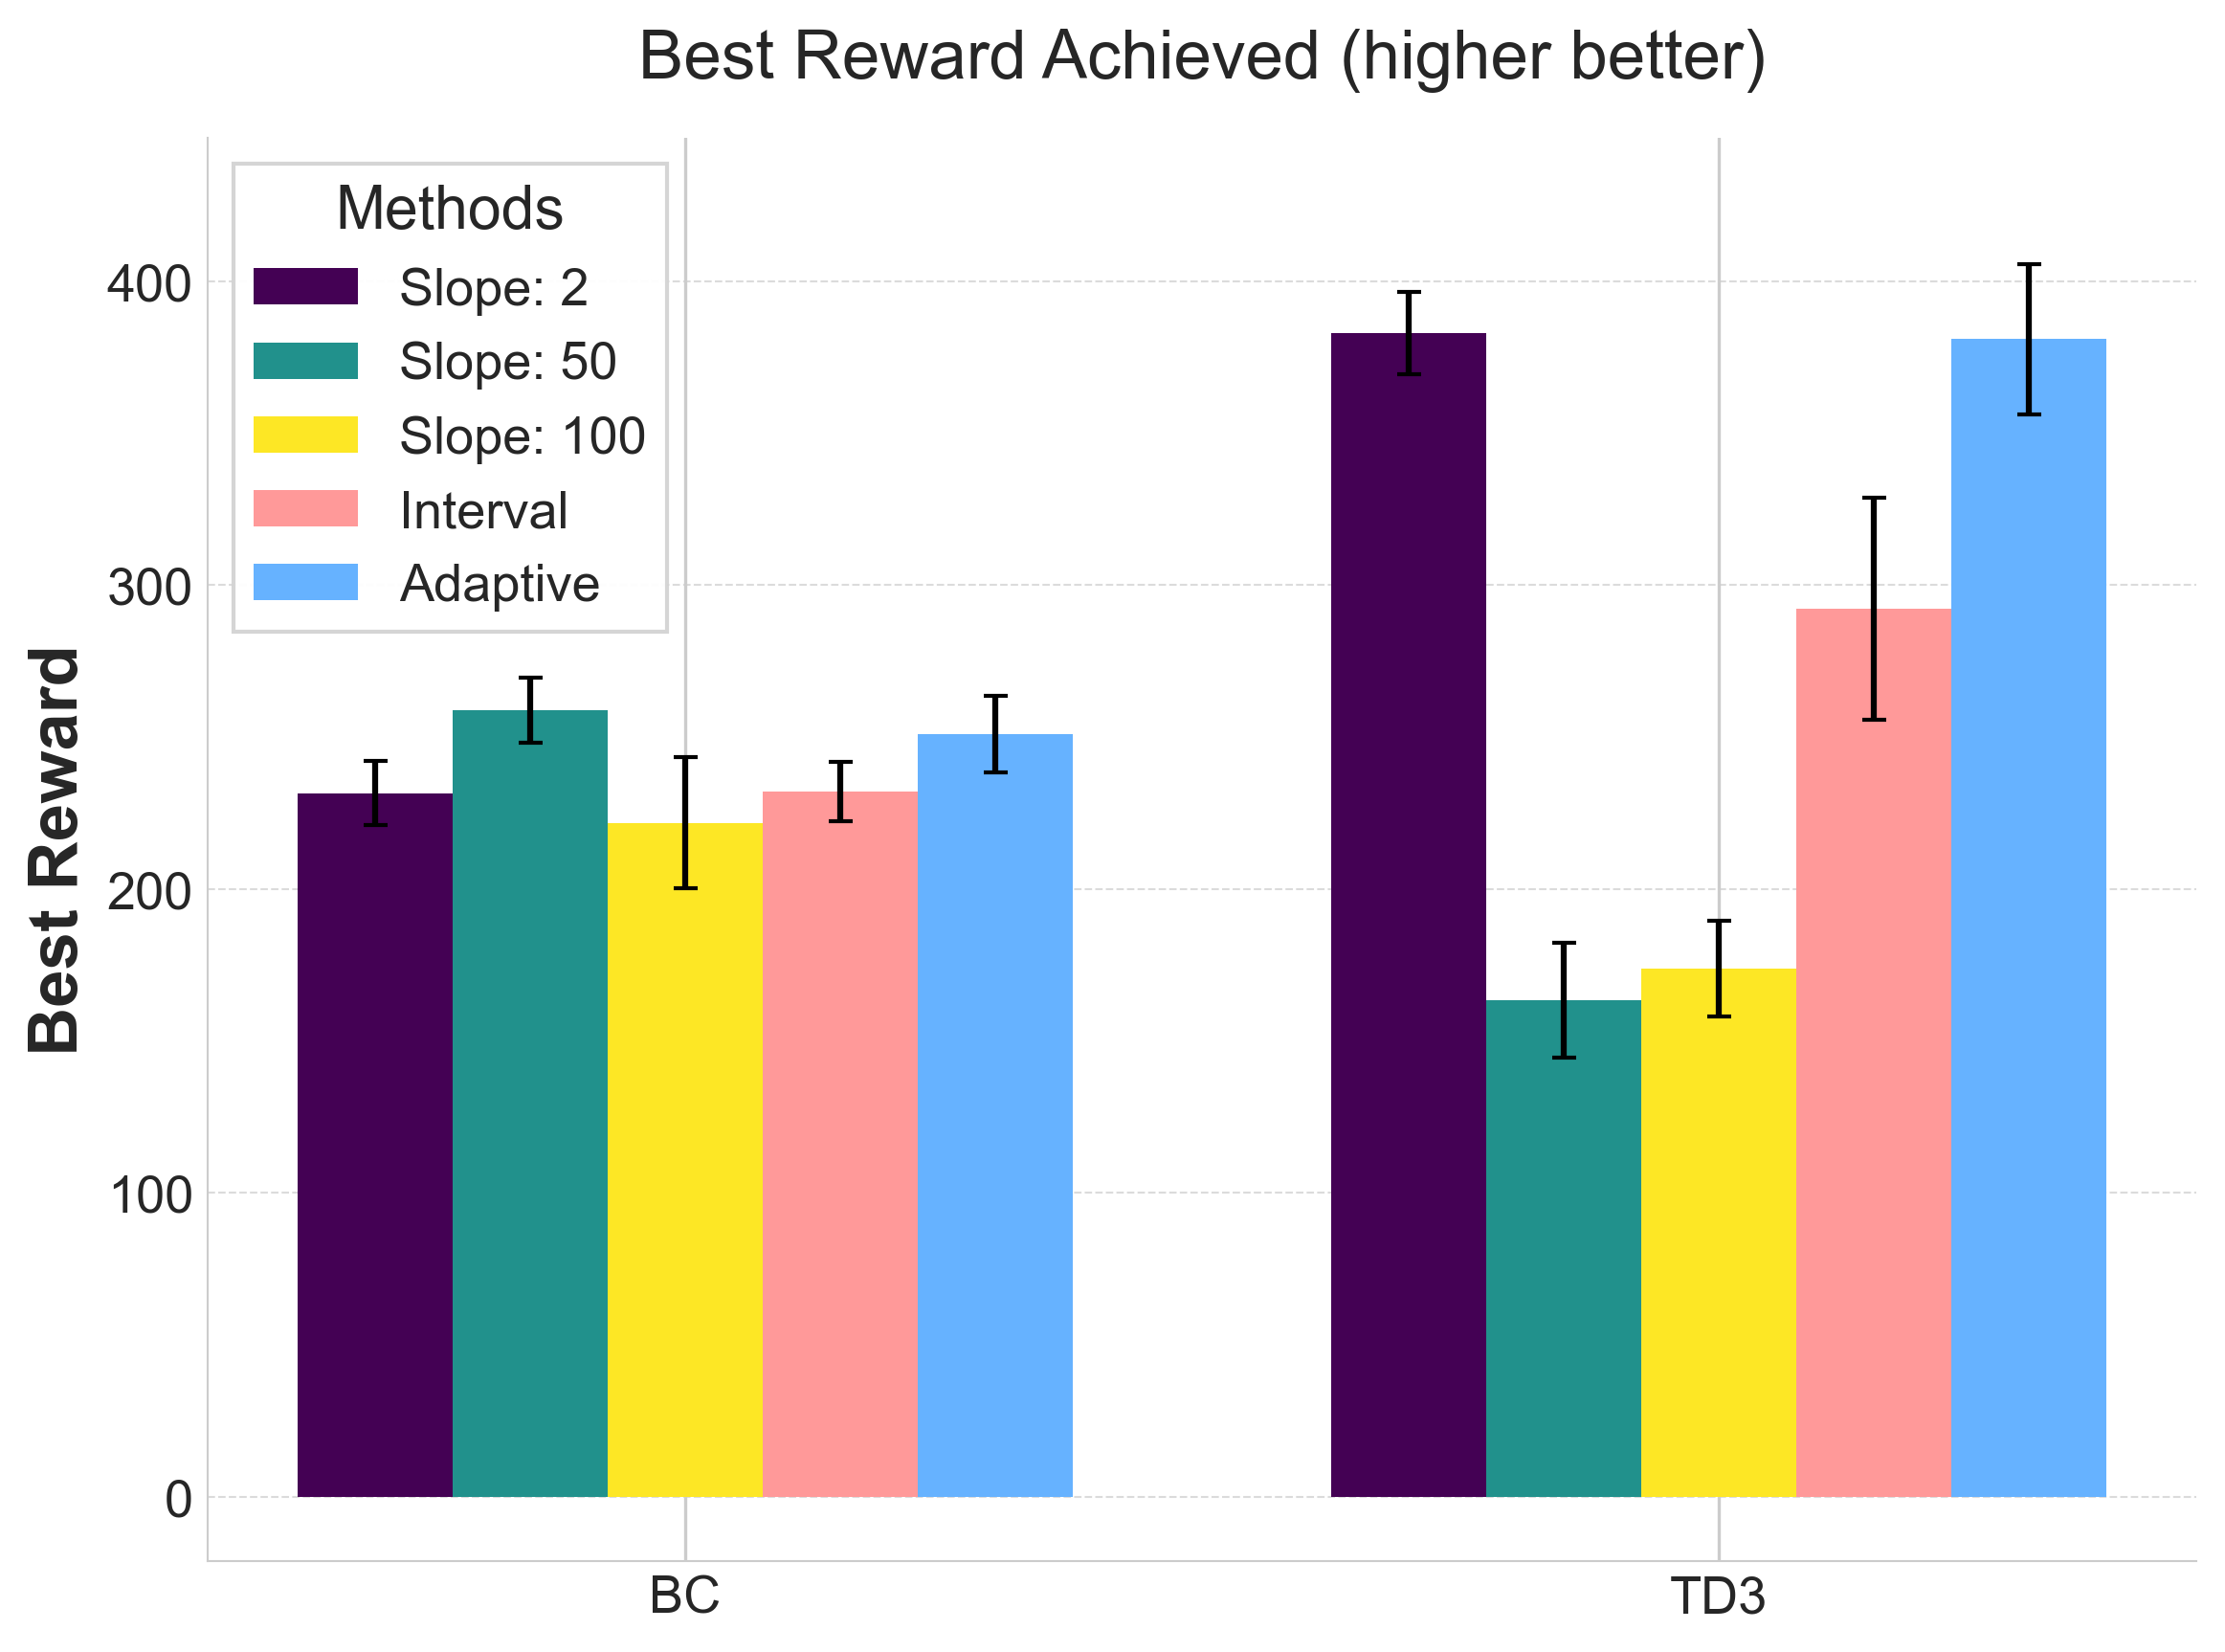
\includegraphics[width=\textwidth]{figures/neurips_best_reward_plot.png}
        \caption{For BC, final performance remains largely invariant to the slope setting, confirming the robustness of supervised training. In RL, however, shallow slopes yield superior asymptotic rewards due to their exploration-promoting noise. Scheduled slopes, specifically adaptive scheduling performs competitively, approaching the performance of optimally tuned shallow slopes while improving training stability. }
        \label{fig:best_reward}
    \end{subfigure}
    \caption{Comparison between fixed and scheduled surrogate gradient slopes for both BC and RL settings. While BC performance is largely slope-invariant, RL benefits from shallower or scheduled slopes, which improve exploration and training efficiency. Scheduling effectively balances stability and performance, reducing the need for extensive slope tuning.}
    \label{fig:fullwidthfigure}
\end{figure*}

While using an interval or adaptive schedule for the surrogate gradient slope does not always result in the best performing network, we find that it can stabilize training. Moreover, it achieves a near-optimal performance on both training speed and final performance. As a result, such schedules eliminate the need for exhaustive hyperparameter sweeps across different slope settings to identify the best performing ones.


\subsection{Training on Sequences with Reward Curriculum}
To fully leverage the temporal processing capabilities of SNNs in RL, we extend training from single transitions to full sequences (\autoref{sub:seq_snn}) and introduce a reward curriculum that gradually increases penalties on position, velocity, and action magnitude to encourage stable, robust behavior. All experiments use an adaptive slope scheduler for surrogate gradient slope adjustment. We compare BC, TD3BC, TD3, and TD3BC+JSRL. BC and TD3BC are offline RL algorithms trained on dataset sequences, gathered with the guiding policy used in our TD3BC+JSRL setup, while TD3 and TD3BC+JSRL are online algorithms sampling sequences from the environment. Unlike TD3, which starts from scratch, TD3BC+JSRL benefits from a privileged guiding policy during the first $n$ steps of rollouts. All approaches are evaluated under the same reward curriculum.
\begin{figure*}[h!]
    \centering
    \begin{subfigure}[b]{0.49\textwidth}
        \centering
        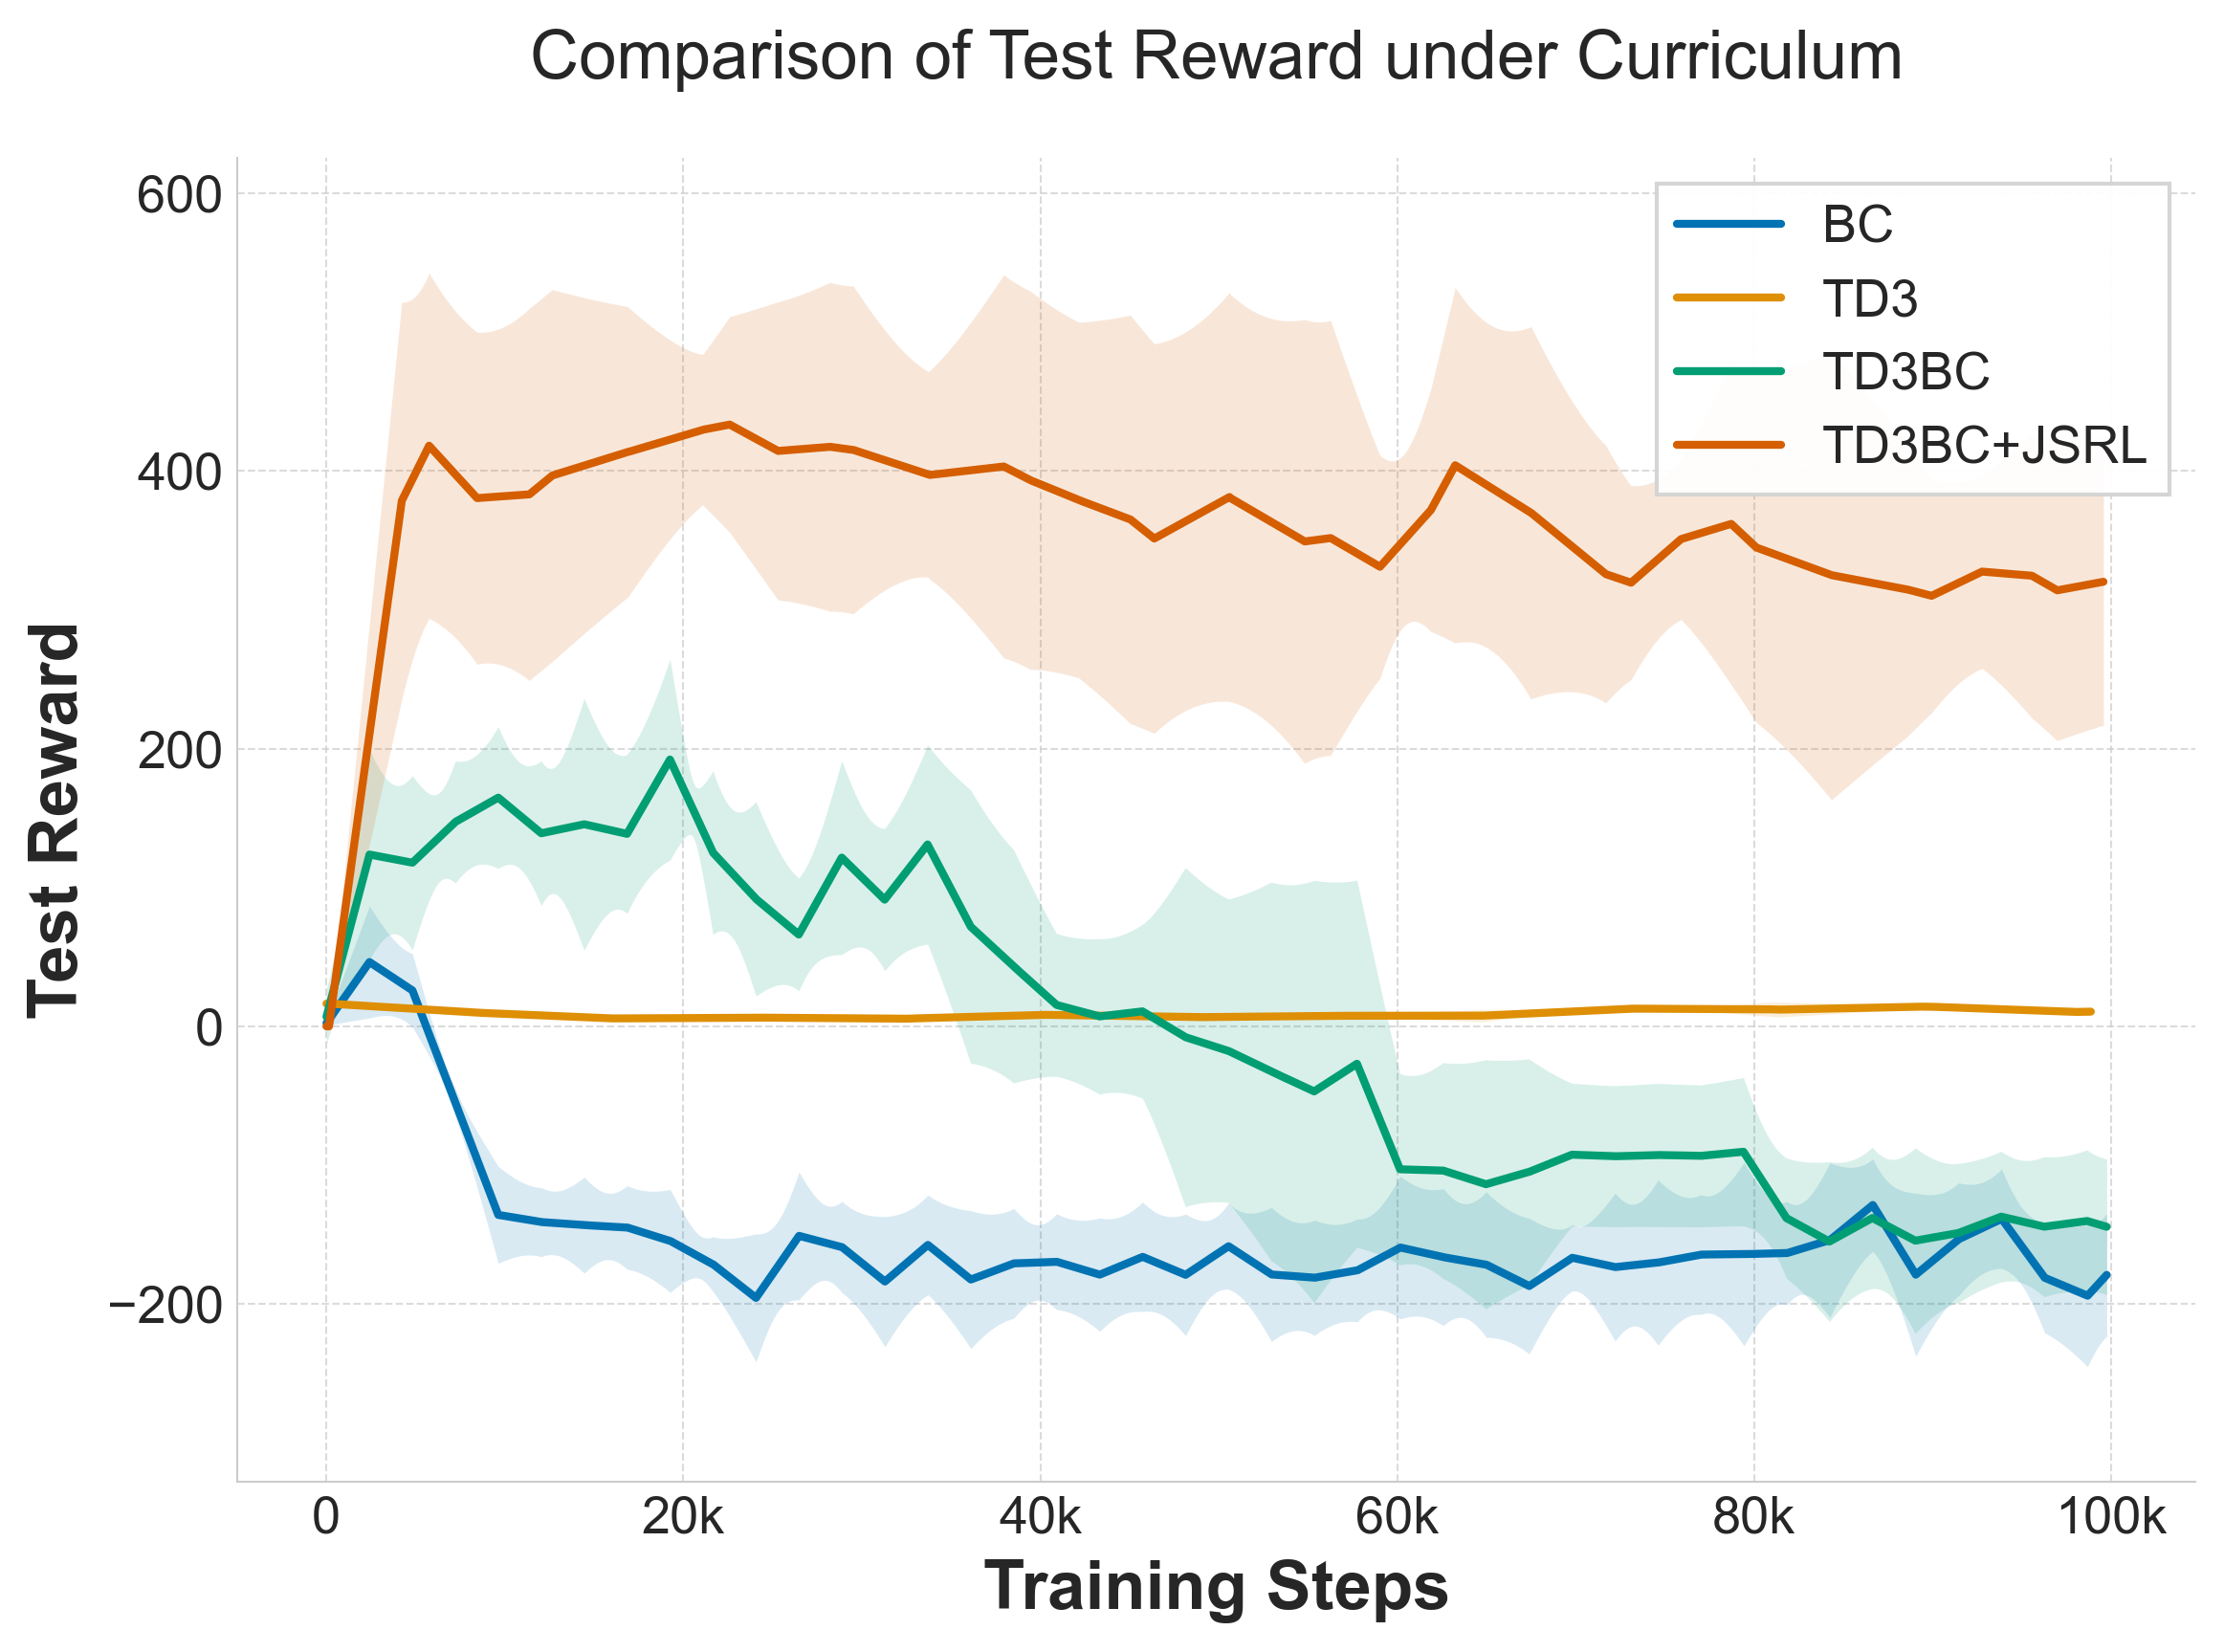
\includegraphics[width=\textwidth]{figures/neurips_comparison_plot_reward.png}
        \caption{Offline methods (BC and TD3BC) struggle as the reward function adapts, failing to generalize beyond the initial dataset, due to the lack of online interactions. TD3BC+JSRL is able to adapt to the curriculum throughout training.}
        \label{fig:rews_training_methods}
    \end{subfigure}
    \hfill
    \begin{subfigure}[b]{0.49\textwidth}
        \centering
        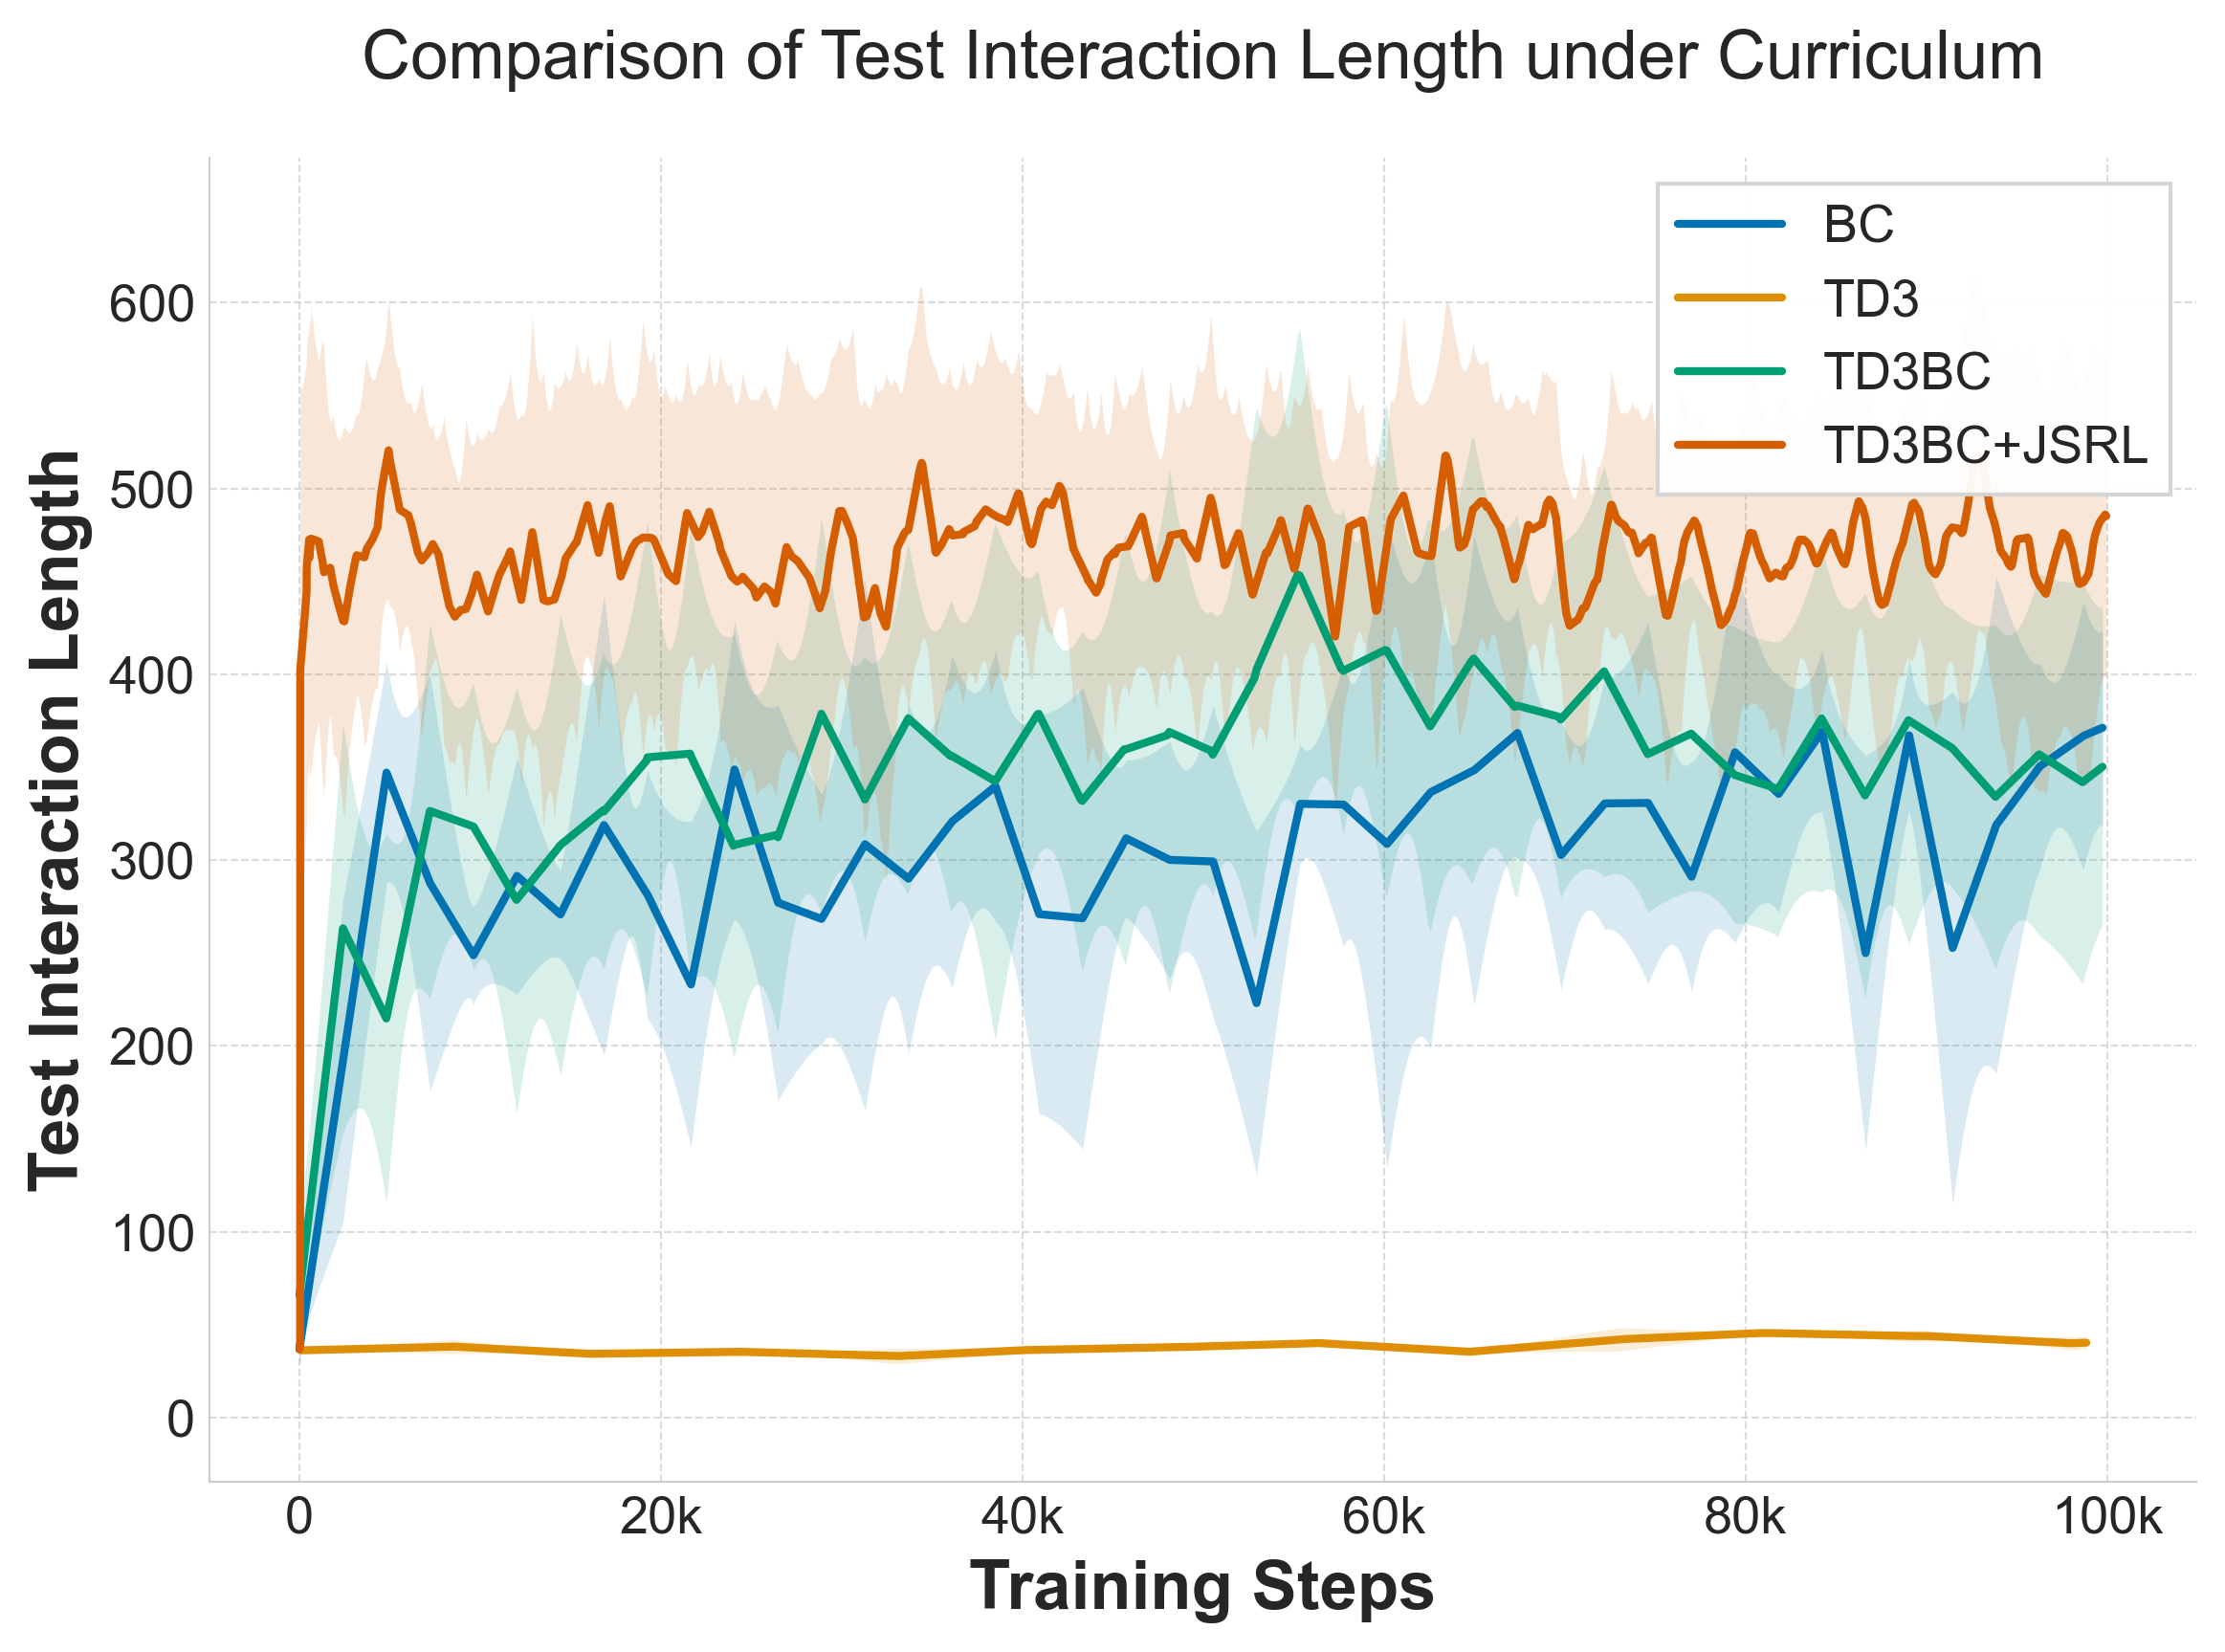
\includegraphics[width=\textwidth]{figures/neurips_comparison_plot_lens.png}
        \caption{While all methods, except TD3, eventually learn to fly, TD3-trained policies frequently terminate early due to unstable exploration. TD3BC+JSRL achieves longer and more stable flight trajectories. 
}
        \label{fig:lens_training_methods}
    \end{subfigure}
    \caption{Comparison of training approaches under a reward curriculum. All experiments were run with 5 different seeds. As the curriculum increases difficulty of the task, we find that only TD3BC+JSRL is able to adapt to the changing curriculum. During testing, we average the results from 20 runs.}
    \label{fig:training-plots}
\end{figure*}

TD3BC+JSRL achieves $400$-point average reward under curriculum learning, while BC, TD3BC, and vanilla TD3 fail to exceed $-200$ points (Figure~\ref{fig:rews_training_methods}). This $600$-point gap validates both components of our approach: leveraging demonstrations (vs. TD3's from-scratch learning) and online adaptation (vs. BC/TD3BC's static datasets).

As the curriculum tightens, BC and TD3BC, trained on static datasets containing rollouts of the guiding actor, fail to generalize, as shown in \autoref{fig:rews_training_methods}. While TD3 has access to evolving interactions, it struggles to gather meaningful sequences early in training, often resulting in premature episode terminations, as seen on \autoref{fig:lens_training_methods}, failing to bridge the warm-up period. Our proposed TD3BC+JSRL approach, which leverages new rollouts guided by the policy, demonstrates robust learning even under a challenging curriculum. The inclusion of online rollouts enables the policy to adapt to the evolving reward landscape, leading to substantial performance improvements. 

The hyperparameters, curriculum and training details used for the experiment are part of the supplementary materials, \autoref{sup:sim}.

\subsection{Bridging the Reality Gap}
We quantitatively evaluated the computational efficiency of our sequential SNN approach using NeuroBench \cite{yik2023neurobench}. 
The trained SNN is compared to a feedforward ANN that achieves similar performance, trained using TD3. This controller requires explicit action history to control the drone successfully. Results show that temporally-trained SNNs match ANN performance while exhibiting distinct computational traits. Despite a higher memory footprint, SNNs benefit from activation sparsity and primarily use energy-efficient accumulates (ACs) instead of energy-hungry multiply-accumulates (MACs), making them well-suited for neuromorphic deployment. While the number of dense operations of the SNN is much higher than the ANN to which we compare, the nature of the underlying ACs opens the opportunity for energy efficient compute. Using the methodology proposed by Davies \textit{et al.} \cite{Davies2018}, we can compute a rough energy consumption estimate of $9.7\times10^{-5}mJ$, see \autoref{sup:energy} for further details.

\begin{table}[h]\label{tab:NeuroBenchResults}
\caption{NeuroBench performance comparison between ANN (64-64 architecture) and temporally-trained SNN (256-128 architecture) using TD3BC+JSRL. While dense operations are computed ignoring activation and connection sparsity, effective operations reflect the sparsity-aware number of operations, as defined in NeuroBench \cite{yik2023neurobench}. }
\centering
\renewcommand{\arraystretch}{1.5}
\begin{tabular}{c|c|c|c|c|c|c|c}
\toprule
Model & \makecell{Reward} & \makecell{Footprint\\(kb)} & \makecell{Activation\\Sparsity} &
\makecell{SynOps\\Dense} & \makecell{SynOps\\Eff\_MACs} &
\makecell{SynOps\\Eff\_ACs} & \makecell{Requires\\History} \\
\midrule
ANN & \textbf{447} & 55.3 & 0.00 & $13.7\times 10^{3}$ & $13.7\times 10^{3}$ & 0.0 & Yes \\
SNN & 446 & 158.3 & 0.79 & $37.9\times 10^{3}$ & $4.6\times 10^{3}$ & $12.2\times 10^{3}$ & No \\
\bottomrule
\end{tabular}
\end{table}


When deployed on the Crazyflie, the SNN controller exhibits slightly oscillatory behavior. However, the SNN is still able to execute complex maneuvers like circles (see \autoref{fig:realCrazyflie}), figure-eight and square trajectories without failure. ANN controllers, benefiting from full action history, show smoother control. However, when comparing to our SNN to an ANN which does not receive action history, we find that the ANN can no longer control the drone, as shown in \autoref{tab:comparison}.

To improve stability, future work could incorporate angular velocity penalties in the reward function, use throttle deviation outputs rather than absolute throttle settings, train for longer, or increased control frequency, as prior work has shown smoother SNN control at higher rates \cite{Eschmann2023,stroobants2025neuromorphic}.
\begin{figure}[]
    \centering
    \includegraphics[width=0.47\textwidth]{figures/CrazyflieFlight.png}
    \caption{When deployed on the Crazyflie, the spiking actor exhibits oscillatory behavior but always successfully performs maneuvers such as circular flight.}

    \label{fig:realCrazyflie}
\end{figure}

Compared to ANN controllers from Eschmann et al. \cite{Eschmann2023}, SNNs trained with our approach achieved lower position error under ideal conditions but had reduced reliability. Notably, while ANNs without action history failed to control the drone. A demonstration video is available online\footnote{\url{https://www.youtube.com/playlist?list=PLAS2CClQ48jX2R-tqza9kRPx0NW1EfKj0}}.

\begin{table}[h]
\caption{Comparison of neural network models for position control and trajectory tracking tasks. The models include an ANN with action history, an ANN without action history and an SNN trained with TD3BC+JSRL without action history. The mean position error of the deployed SNNs is benchmarked against the best-performing ANN policy \cite{Eschmann2023}. Position error is measured as the average xy-plane error (in meters), and trajectory tracking error is evaluated as the average error across figure-eight and square-following tasks. The ANN without action history did not manage to stabilize the quadrotor. }
\centering
\renewcommand{\arraystretch}{1.5}
\begin{tabular}{c|c|c|c|c} 
& \makecell{ANN\\action history \cite{Eschmann2023}} & \makecell{ANN\\no action history \cite{Eschmann2023}} & \makecell{SNN\\no action history [Ours]}  \\ \hline
\makecell{Position Error [m]} & 0.1 & 0.25 & 0.04 \\\hline
\makecell{Trajectory Error [m]} & 0.21 & NA & 0.24 \\ 
\end{tabular}

    \label{tab:comparison}
\end{table}

\subsection{Ablation Study}
To analyze the contribution of each component of the algorithm, an ablation study is performed. We first remove only the BC-term, then only the jump-start period. Lastly, we analyze the result with no BC-term and no Jump-Start. 

Removing the BC term allows the SNN controller to eventually show improvements in performance, but convergence becomes substantially slower, approximately $15$ times more training steps are required to achieve a reward of $100$. In contrast, eliminating the jump-starting actor entirely prevents the SNN from collecting sequences long enough to bridge the warm-up period, resulting in the network failing to learn stable flight altogether. As expected, removing both terms, leads to similar behavior. We find the BC term to improve training efficiency when the jump-start period allows bridging the warm-up period, and fills the buffer with several demonstrations from the guiding policy.
\begin{table}[h!]
\centering
\caption{Ablation study analyzing the impact of the BC-term and Jump-Start period on training performance. Reported values show the average final reward and the number of environment steps required to reach a reward of $100$.}
\label{tab:ablation}
\begin{tabular}{lcccc}
\toprule
\textbf{BC-term} & \textbf{Jump-start}  & \textbf{Reward} & \textbf{Steps to 100} \\
\midrule
Yes & Yes &  $412 \pm 6.72$ & $2200 \pm 124$  \\
No & Yes & $334 \pm 25.59$ & $33030 \pm 1600$ \\
Yes & No & $32 \pm 1.2$ &  NA\\
No & No & $36 \pm 4.1$  & NA \\
\bottomrule
\end{tabular}
\end{table}
